% file: 3-5-mst/spanning-tree.tex

\documentclass[tikz]{standalone}

\usetikzlibrary{positioning}

\begin{document}
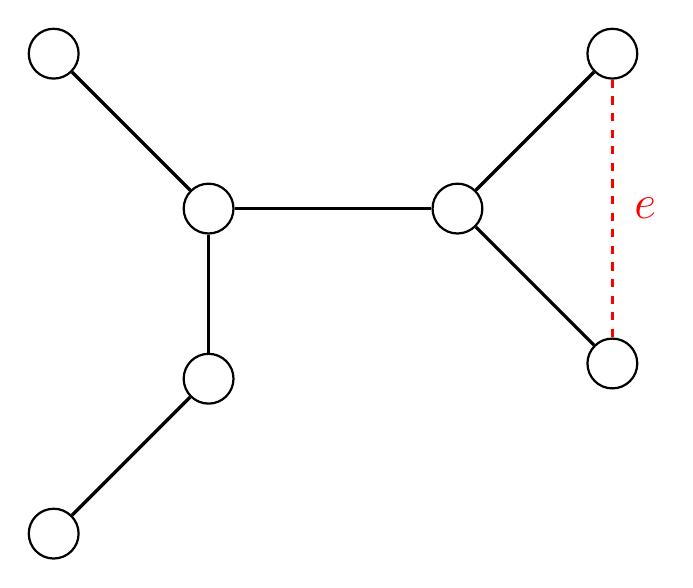
\begin{tikzpicture}[tnode/.style = {circle, draw, thick, minimum size = 18pt},
  every edge/.style = {draw, very thick},
  node distance = 1.5cm and 1.5cm]
  \node (1) [tnode] {};
  \node (2) [tnode, right = 2.5cm of 1] {};
  \node (3) [tnode, above right = of 2] {};
  \node (4) [tnode, below right = of 2] {};
  \node (5) [tnode, below = of 1] {};
  \node (6) [tnode, below left = of 5] {};
  \node (7) [tnode, above left = of 1] {};

  \path (1) edge (2)
  	    edge (5)
	    edge (7)
  	(2) edge (3)
	    edge (4)
	(5) edge (6)
	(3) edge[red, dashed] node [right = 4pt, font = \LARGE] {$e$} (4);
\end{tikzpicture}
\end{document}
